\section{Модель рассеяния электронного пучка в системе ПММА/Si}

Для моделирования рассеяния электронного пучка в системе ПММА/Si в данной работе был реализован алгоритм на основе метода Монте-Карло.
Для описания процессов упругого рассеяния использовались моттовские сечения упругого рассеяния, рассчитанные с использованием свободно распространяемой программы ``ELSEPA''~\cite{ELSEPA}.
Для описания процессов неупругого рассеяния электронного пучка в ПММА была использована модель, учитывающая электрон-электронное, электрон-фононное и электрон-поляронное рассеяние~\cite{Ciappa_2010}. Для описания процессов неупругого рассеяния в кремнии использовался подход, в котором функция потерь энергии вещества представляется в виде суммы функций потерь энергии осцилляторов Друде с квадратичным законом дисперсии~\cite{Valentin2012_Si}.
Данный алгоритм позволил промоделировать акты электрон-электронного рассеяния в \linebreak ПММА, распределение которых в дальнейшем использовалось для моделирования распределения электронно-стимулированных разрывов молекул ПММА.

\section{Модель электронно-стимулированных разрывов молекул ПММА}
Для моделирования электронно-стимулированных разрывов молекул \linebreak ПММА был разработан подход, основанный на предположении, что разрыв молекулы происходит при электрон-электронном рассеянии с вероятностью $\ps$.
В этом случае экспериментально наблюдаемое увеличение радиационно-химического выхода разрывов $\Gs$ с ростом температуры может быть описано за счет увеличения $\ps$.
Для нахождения зависимости $\ps$ от температуры было проведено моделирование эксперимента по определению $\Gs$ на основе значений среднечисловой молекулярной массы резиста до и после экспонирования.
Параметры эксперимента были взяты из работы~\cite{Harris_G_value}: толщина слоя ПММА -- 500~нм, энергия электронного пучка -- 10 кэВ, доза экспонирования -- 100 мкКл/см$\pp$. Начальные значения среднечисловой и средневесовой молекулярной массы ПММА составляли 563000 и 2260000 соответственно.

Для моделирования среднечисловой молекулярной массы проэкспонированного ПММА была специально разработана модель слоя ПММА, предоставляющая подробную информацию о молекулярно-массовом распределении \linebreak ПММА.
Изначально на основе модели идеальной цепи~\cite{Han_2003} были промоделированы отдельные молекулы, длины которых согласовывались с начальным молекулярно-массовым распределением ПММА~\cite{Harris_G_value}.
Далее для каждой молекулы случайным образом выбиралось положение внутри области размерами 100$\times$100$\times$500 нм$\ppp$ с учетом периодических граничных условия.
Область заполнялась молекулами до тех пор, пока не была достигнута необходимая плотность (1.19 г/см$\ppp$) (рисунок~\ref{fig:Harris_chains}).

\begin{figure}[t!]
	\begin{minipage}{0.48\textwidth}
		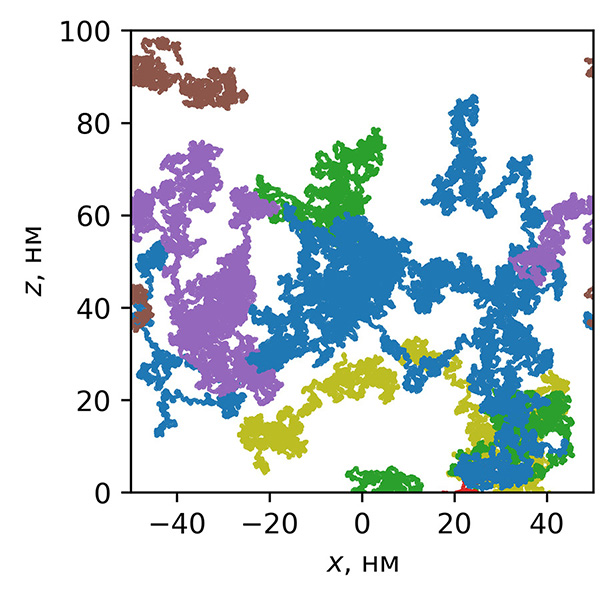
\includegraphics[width=0.95\linewidth]{G_value/Harris_chains_1step_200}
		\vspace{-14.2em} \\ \text{\hspace{0em} a}) \\ \vspace{14.2em}
	\end{minipage}
	\begin{minipage}{0.48\textwidth}
		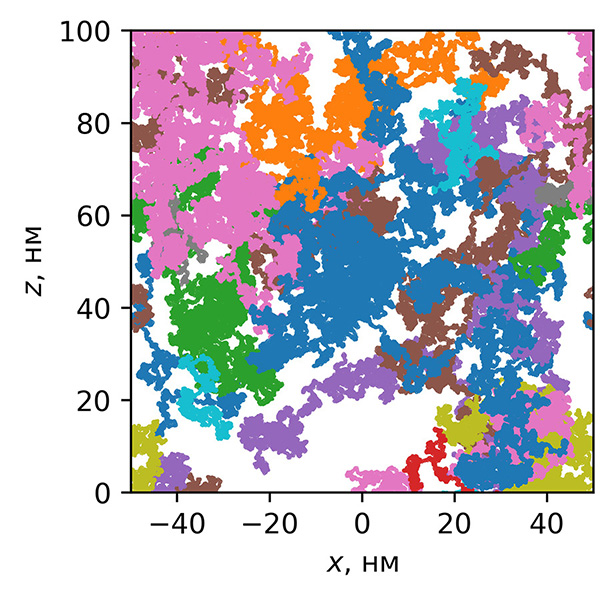
\includegraphics[width=0.95\linewidth]{G_value/Harris_chains_2step_200}
		\vspace{-14.2em} \\ \text{\hspace{0em} б}) \\ \vspace{14.2em}
	\end{minipage}
	\vspace{-3.5em}
	\begin{center}
		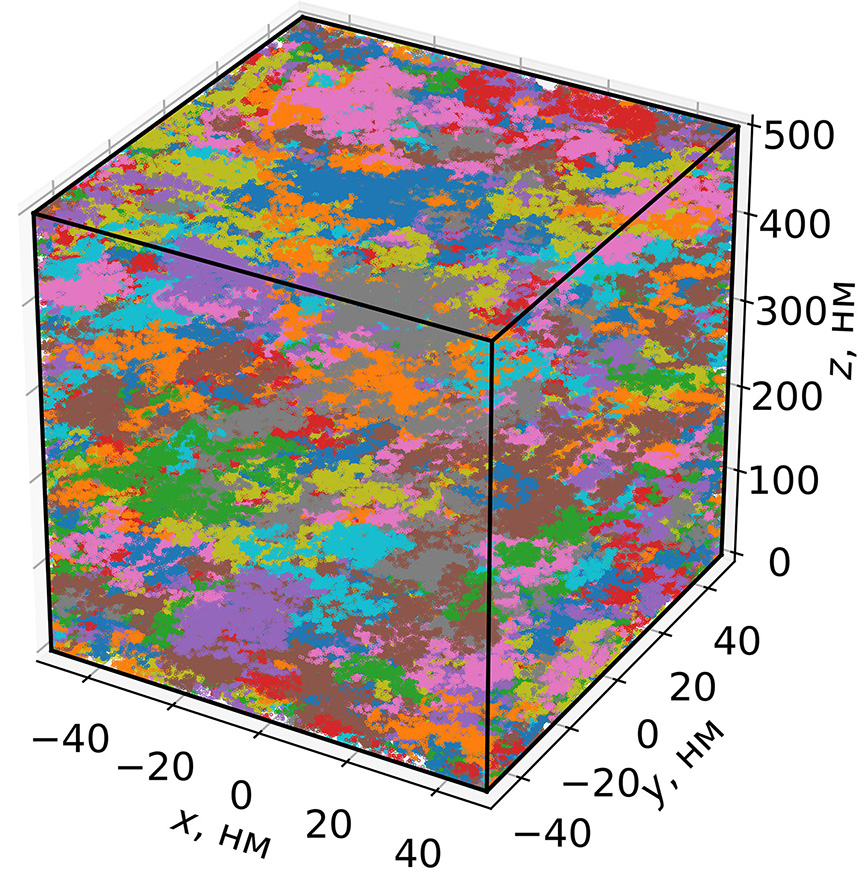
\includegraphics[width=0.5\linewidth]{G_value/Harris_chains_14_200}
		\vspace{-13em} \\ \text{\hspace{-20em} в}) \\ \vspace{13em}
	\end{center}
	\vspace{-1.5em}
	\caption{Иллюстрация процесса заполнения области моделями молекул ПММА (а, б) при моделировании слоя ПММА (в).}
	\label{fig:Harris_chains}
\end{figure}

Дальнейшее моделирование рассеяния электронного пучка в системе в системе ПММА/Si проводилось в предположении о равномерном распределении дозы экспонирования по площади для участка размерами 100$\times$100~нм$\pp$ с периодическими граничными условиями.
После этого область, занимаемая молекулами ПММА, разделялась на ячейки размерами 5$\times$5$\times$5 нм$\ppp$, и для каждой ячейки определялось соответствующее ей число промоделированных актов электрон-электронного рассеяния $N_{\mathrm{e-e}}[i, j, k]$.
Для каждого акта электрон-электронного рассеяния моделировалось, будет ли он приводить к разрыву молекулы ПММА или нет:
\begin{equation} \label{eq:MC_9}
	\begin{aligned}
		\xi < p_\mathrm{s} & \Rightarrow \text{разрыв молекулы} \\
		\xi \geq p_\mathrm{s} & \Rightarrow \text{нет разрыва},
	\end{aligned}
\end{equation}
где $\xi$ -- случайное число из промежутка [0, 1).
Таким образом, задание $p_\mathrm{s}$ позволяло промоделировать число разрывов в каждой ячейке слоя ПММА $N_\mathrm{s}[i, j, k]$.
Далее для каждой ячейки определялось, мономеры каких молекул находились в ней, и среди них случайным образом выбирались $N_\mathrm{s}[i, j, k]$ мономеров, которым сопоставлялись разрывы.
Учитывая тот факт, что номера молекул, проходящих через каждую ячейку, а также положения мономеров, входящих в каждую молекулу, хранились в памяти компьютера, такой подход позволял определить положения разрывов в каждой молекуле, входящей в модель слоя ПММА.
При известных положениях разрывов в каждой молекуле среднечисловая молекулярная масса проэкспонированного ПММА определялась непосредственным образом, и экспериментальное значение $\Gs$ рассчитывалось по формуле~\ref{eq:G_value_Mn_Mf}.

Экспериментальная зависимость $\Gs(T)$, приведенная в работе~\cite{Charlesby_1964_Gs}, была аппроксимирована функцией
\begin{equation}
	\ln(\Gs) = \frac{k}{T} + b,
\end{equation}
в результате чего были получены значения -454.012 и 2.008 для параметров $k$ и $b$ соответственно.
За счет этого были получены экспериментальные значения $\Gs$ для температур из диапазона 0--200~$^\circ$C, и для каждой температуры было подобрано значение $\ps$ обеспечивающее равенство между промоделированным и экспериментальным значениями $\Gs$ (``моделирование $\Gs$'' на рисунке~\ref{fig:P_s}).

Также, в качестве альтернативного подхода температурная зависимость $\ps$ была рассчитана непосредственно из определения $\Gs$ как числа разрывов, приходящегося на 100 эВ выделившейся в резисте энергии (``теоретическое $\Gs$'' на рисунке~\ref{fig:P_s}).
Явное различие между графиками, отображающими каждую из зависимостей, указывает на целесообразность моделирования молекулярно-массового распределения ПММА для определения $\ps$.

В таблице~\ref{table:p_s} приведены значения $\ps$, полученные для температур 130, 140 и 150~$^\circ$C при проведении пяти независимых моделирований.
Разброс значений для каждой температуры составляет менее 1\% от среднего значения, в силу чего было принято решение пренебречь статистической погрешностью $\ps$.

\begin{figure}[h]
	\centering
	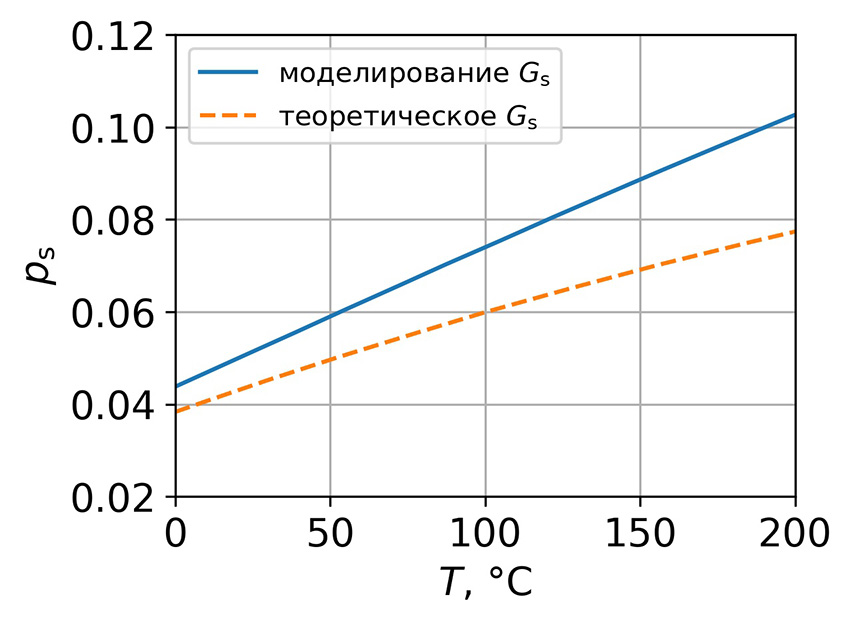
\includegraphics[width=0.55\linewidth]{G_value/G_s_14_200}
	\caption{Рассчитанная температурная зависимость вероятности разрыва $\ps$ молекулы ПММА при электрон-электронном взаимодействии (график ``моделирование $\Gs$''). График ``теоретическое $\Gs$'' отображает аналогичную зависимость, полученную непосредственно из определения величины $\Gs$.\vspace{1.5em}}
	\label{fig:P_s}
\end{figure}

\begin{table}[h]
	\caption{Значения вероятности разрыва молекулы ПММА при электрон-электронном взаимодействии для различных температур, полученные в пяти независимых моделированиях.}
	\begin{center}
		\begin{tabular}{c c r c r c r}
			\hline \hline \\[-1em]
			Номер моделирования & \hspace{0em} & $\ps$ при 130~$^\circ$C & \hspace{0em} & $\ps$ при 140~$^\circ$C & \hspace{0em} & $\ps$ при 150~$^\circ$C \\ \hline
			\\ [-1em]
			1 & \hspace{0em} & 8.2844\:$\cdot$\,10$^\text{-2}$ & \hspace{0em} & 8.5752\:$\cdot$\,10$^\text{-2}$ & \hspace{0em} & 8.8647\:$\cdot$\,10$^\text{-2}$
			\\ \\ [-1em]
			2 & \hspace{0em} & 8.3084\:$\cdot$\,10$^\text{-2}$ & \hspace{0em} & 8.6012\:$\cdot$\,10$^\text{-2}$ & \hspace{0em} & 8.8897\:$\cdot$\,10$^\text{-2}$
			\\ \\ [-1em]
			3 & \hspace{0em} & 8.2829\:$\cdot$\,10$^\text{-2}$ & \hspace{0em} & 8.5715\:$\cdot$\,10$^\text{-2}$ & \hspace{0em} & 8.8526\:$\cdot$\,10$^\text{-2}$
			\\ \\ [-1em]
			4 & \hspace{0em} & 8.2834\:$\cdot$\,10$^\text{-2}$ & \hspace{0em} & 8.5734\:$\cdot$\,10$^\text{-2}$ & \hspace{0em} & 8.8606\:$\cdot$\,10$^\text{-2}$
			\\ \\ [-1em]
			5 & \hspace{0em} & 8.2987\:$\cdot$\,10$^\text{-2}$ & \hspace{0em} & 8.5880\:$\cdot$\,10$^\text{-2}$ & \hspace{0em} & 8.8797\:$\cdot$\,10$^\text{-2}$
			\\ \hline \hline
		\end{tabular}
		\label{table:p_s}
	\end{center}
\end{table}
